\chapter{Hybrid Control}
\label{ch:Hybrid Control}

The hybrid control is a control method that comprises more than one sensor type. The one that will be applied to this work will use force sensors attached to the arm of the exoskeleton. 

The values measured by the sensors will define a dynamic area. We define dynamic area as a set of a number of activities to be performed based on a set of combinations from the readings of the sensors. It is based on the dynamic area proposed by Philipson \cite{Philipson1985} shown in figure \ref{Movement space}
The control will be based in a dynamic area composed of three levels for each of the sensors: The sEMG sensor and the force sensor (figure \ref{DynamicAreaHybrid}). The convention for the force sensor signal is positive for when the user is applying a force to the exoskeleton in the direction of the flexion movement and negative in the direction of extension movement. The sEMG sensor is placed at the muscle responsible for the flexion movement.

\begin{figure}[thpb]
      \centering
      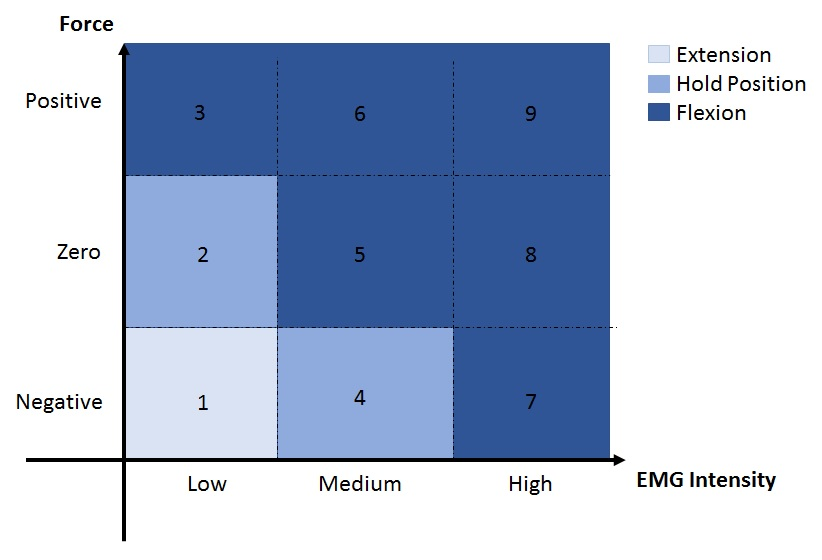
\includegraphics[scale=0.6]{Images/DynamicAreaHybrid.jpg}
      \caption{Dynamic area for the hybrid control.}
      \label{DynamicAreaHybrid}
   \end{figure}

The dynamic area shows the desired motion for the mechanism according to the level of the inputs from both sensors.

Each area, denoted by a number in the figure, represents a different situation for the user. The reasoning behind the decision making of the controller is as follows:

\begin{itemize}
\item 1: No movement intention but there is a load forcing the limb to an extension movement.
\item 2: There is no movement intention nor load forcing the limb to extension or flexion movement.
\item 3: The user is flexing his limb and supporting the entirety of the load as well as forcing the exoskeleton to a flexion movement.
\item 4: User has the intention to maintain his limb position and its arm is being supported by the exoskeleton.
\item 5: The user's strength is in equilibrium with the weight of the load, but the exoskeleton must act to support the user's arm, avoiding fatigue.
\item 6: Same as 3
\item 7: Intention of movement, but the user is unable to lift the load using his own strength.
\item 8: Intention of movement, but the user's strength is in equilibrium with the weight of the load.
\item 9: The user is carrying the weight by himself and forcing the exoskeleton in the flexion direction.
\end{itemize}

This way it is possible to implement a set of rules for the controller:

If the signal from the sEMG is low, there is no intention of movement from the user. This way, the user's limb offers no resistance to external loads. If any external load is applied the user's limb will move in the same direction as the force applied and the exoskeleton should move in that same direction, offering no resistance.

If the signal from the sEMG is in an intermediate level, it characterizes the user's intention to maintain its limb position. If the force sensor measures a negative force, the exoskeleton is supporting the user's limb. Therefore, it must maintain its position. If the force sensor measures no force, the user is carrying the load using his own strength, potentially causing muscular fatigue. The exoskeleton must act in the extension direction until it supports the user's limb, maintaining a comfortable position for the user. When the force sensor measures a positive force, the user's limb is supporting the entirety of the load and forcing the exoskeleton into a flexion movement. The exoskeleton perform a flexion movement to alleviate the load applied to the user's limb.

If the signal from the sEMG is high, it characterizes a movement intention from the user. If the force sensor measures a negative force, the user's strength is inferior to the load, so the exoskeleton must assist the user's movement. If the force sensor measures no force, the user's strength is sufficient to maintain the limb in a static position, but it will soon cause fatigue. The exoskeleton must act to support the user's limb and the load. If the force sensor measures a positive force, the user is carrying the load and forcing the exoskeleton in to a flexion movement. The exoskeleton must act to alleviate the load in the user's limb.